% Metódy inžinierskej práce

\documentclass[10pt,oneside,slovak,a4paper,hidelinks]{article}

\usepackage[slovak]{babel}
%\usepackage[T1]{fontenc}
\usepackage[IL2]{fontenc} % lepšia sadzba písmena Ľ než v T1
\usepackage[utf8]{inputenc}
\usepackage{graphicx}
\usepackage{url} % príkaz \url na formátovanie URL
\usepackage{hyperref} % odkazy v texte budú aktívne (pri niektorých triedach dokumentov spôsobuje posun textu)
\usepackage{indentfirst}
\usepackage{color,soul}

\usepackage{cite}
%\usepackage{times}
\graphicspath{ {./res/} }

\pagestyle{headings}

\title{3D Game Engine-y a ich význam\thanks{Semestrálny projekt v predmete Metódy inžinierskej práce, ak. rok 2022/23, vedenie: Zuzana Špitálová}} % meno a priezvisko vyučujúceho na cvičeniach

\author{Jan Lenhart\\[2pt]
	{\small Slovenská technická univerzita v Bratislave}\\
	{\small Fakulta informatiky a informačných technológií}\\
	{\small \texttt{xlenhart@stuba.sk}}
}

\date{\small 30. október 2022} % upravte

\begin{document}
	
	\maketitle
	
	\vspace*{\fill}
	\begin{abstract}
		Každodenným vývojom technológie sa posúvajú aj technologické hranice video hier. V októbri 1958 fyzik William Higinbotham vytvoril, čo sa považuje ako prvá video hra. Bolo to niečo podobné hre PONG. Neskôr v roku 1980 bola vyvinutá prvá 3D hra. Bola to tanková hra, ktorá využívala vektorovú grafiku na 3D realizáciu. Obe tieto hry mali veľký význam pre gamifikáciu a ako sa blížime k dnešnej dobe, tvorba hier začína byť o dosť zložitejšia, preto na jej uľahčenie vznikli game enginy. game enginy nám umožňujú vyvíjať hry ako také, bez toho, aby sme museli míňať čas na vývoj základných prostriedkov na ktorých je založená každá video hra. Týmto vieme, že aj game enginy majú mimoriadne veľký význam pre gamifikáciu. V tomto článku sa dozviete o kľúčových častiach Game enginov, nástrojov na tvorbu zábavných, ale aj edukačných video hier.
	\end{abstract}
	\vspace*{\fill}
	
	\pagebreak
	
	\section{Úvod}
		V dnešnej dobe veľké množstvo ľudí si radi zahrajú nejakú hru vo voľnom čase. Faktom je že štandardy video hier postupne rastú. Už nestačí, aby video hra bola len zábavná, ale aby zanechala aj príjemný dojem. To sa dá dosiahnuť vysoko kvalitnou grafikou, špeciálnymi efektmi, realistickou fyzikou, zvukom a animáciou. Kvôli vysokým štandardom tvorba vysoko kvalitných hier je dôležitá. Práve preto veľkú časť vývojového procesu nám uľahčujú game enginy. Bez nich by tvorba hier rovnakej kvality trvala nesmierne dlho a práve preto takmer všetky video hry, či už vydané AAA štúdiami alebo samostatnými vývojármi sú tvorené pomocou game enginov.
		\paragraph{Čo je game engine?} Game engine je softvér primárne určený na vývoj video hier a vo všeobecnosti zahŕňa príslušné knižnice a podstatné programy. Terminológia engine znamená motor, čiže game engine poháňa hry, alternatívne herný nástroj. Oba tieto preklady sú nepresné a preto v tomto článku je používaný iba výraz game engine z anglického jazyka.
	\subsection{Moderné game enginy}
		V súčasnosti game enginy sa delia na verejné a súkromné. O súkromných vieme veľmi málo, lebo ich vlastnia korporácie na tvorbu ich video hier. Príklad takýchto herných enginov je Rockstar Advanced Game Engine od korporácie Rockstar. Najznámejšie hry vytvorené v tom hernom engine je Grand Theft Auto(GTA). Ďalší známi súkromný game engine je RED Engine, využívaný na hru Cyberpunk 2077, jedna s hier s najlepšou grafikou.
		\paragraph{}Okrem súkromných game enginov sú aj verejné. Medzi najznámejšie verejné herné enginy patria Unreal Engine a Unity Engine. Unreal je od spoločnosti Epic Games, a je veľmi známi pre vysokokvalitnú grafiku a bol používaný v hre Fortnite, Bioshock, Fall Guys a iných. Unity Engine je známi pre svoju kompatibilitu s rôznymi platformami a pre veľmi jednoduchú tvorbu hier. Známe Unity Engine hry sú Pokemon Go, Cuphead a mnohé iné.
		\paragraph{}Napriek tomu že oba tieto herné enginy sú rovnako známe, majú veľký rozdiel v počte hier vytovených v nich. V tabuľke môžete všimnúť tieto rozdiely, ale aj používanosť iných verejných enginov:
		\hspace*{\fill}
		\begin{center}
			\begin{tabular}{|p{5cm}|p{5cm}|}
				\hline
				Názov & Pomer počtu hier\\
				\hline\hline
				Unity		& 47.30\%\\
				Construct	& 12.30\%\\
				GameMaker	& 11.00\%\\
				Twine		& 6.20\%\\
				RPG Maker	& 3.90\%\\
				Bitsy		& 3.30\%\\
				PICO-8		& 2.90\%\\
				Unreal		& 2.80\%\\
				Godot		& 2.50\%\\
				Ren'Py		& 2.00\%\\
				Ostatné game engine-y	& 5.80\%\\
				\hline
			\end{tabular}
		\end{center}
		\paragraph{}Je to kvôli ich licenčným podmienkam. Unity aj Unreal Engine sú k dispozícii pre vývojárov na základe licenčnej zmluvy. Unreal Engine má tolerantnejší licenčný model ako Unity, pretože je k dispozícii na bezplatné používanie s 5\% licenčným poplatkom z hrubého príjmu po prvých 3 000 dolároch za hru za štvrťrok. Unity na druhej strane ponúka bezplatnú osobnú verziu enginu, no vývojári, ktorí ju chcú využívať na komerčné účely, si musia zakúpiť licenciu. Náklady na licenciu Unity sa líšia v závislosti od typu organizácie a príjmov generovaných hrou, ale zvyčajne sa pohybujú od 400 do 150 000 dolárov ročne.
	\section{Systémová architektúra}
		Systémová architektúra game enginov sa dá rozdeliť do dvoch veľkých skupín. Sú to časti nízkej úrovne a časti vysokej úrovne \cite{Primary}. Časti vysokej úrovne sú rozhrania založené na abstrakcii príkazov nízkej úrovne. Na druhej strane časti nízkej úrovne sú menšie systémy, ktoré pomáhajú častiam vysokej úrovne. Pracujú s dátami, dátovými štruktúrami, I/O rozhraniami a správou hardvéru.
		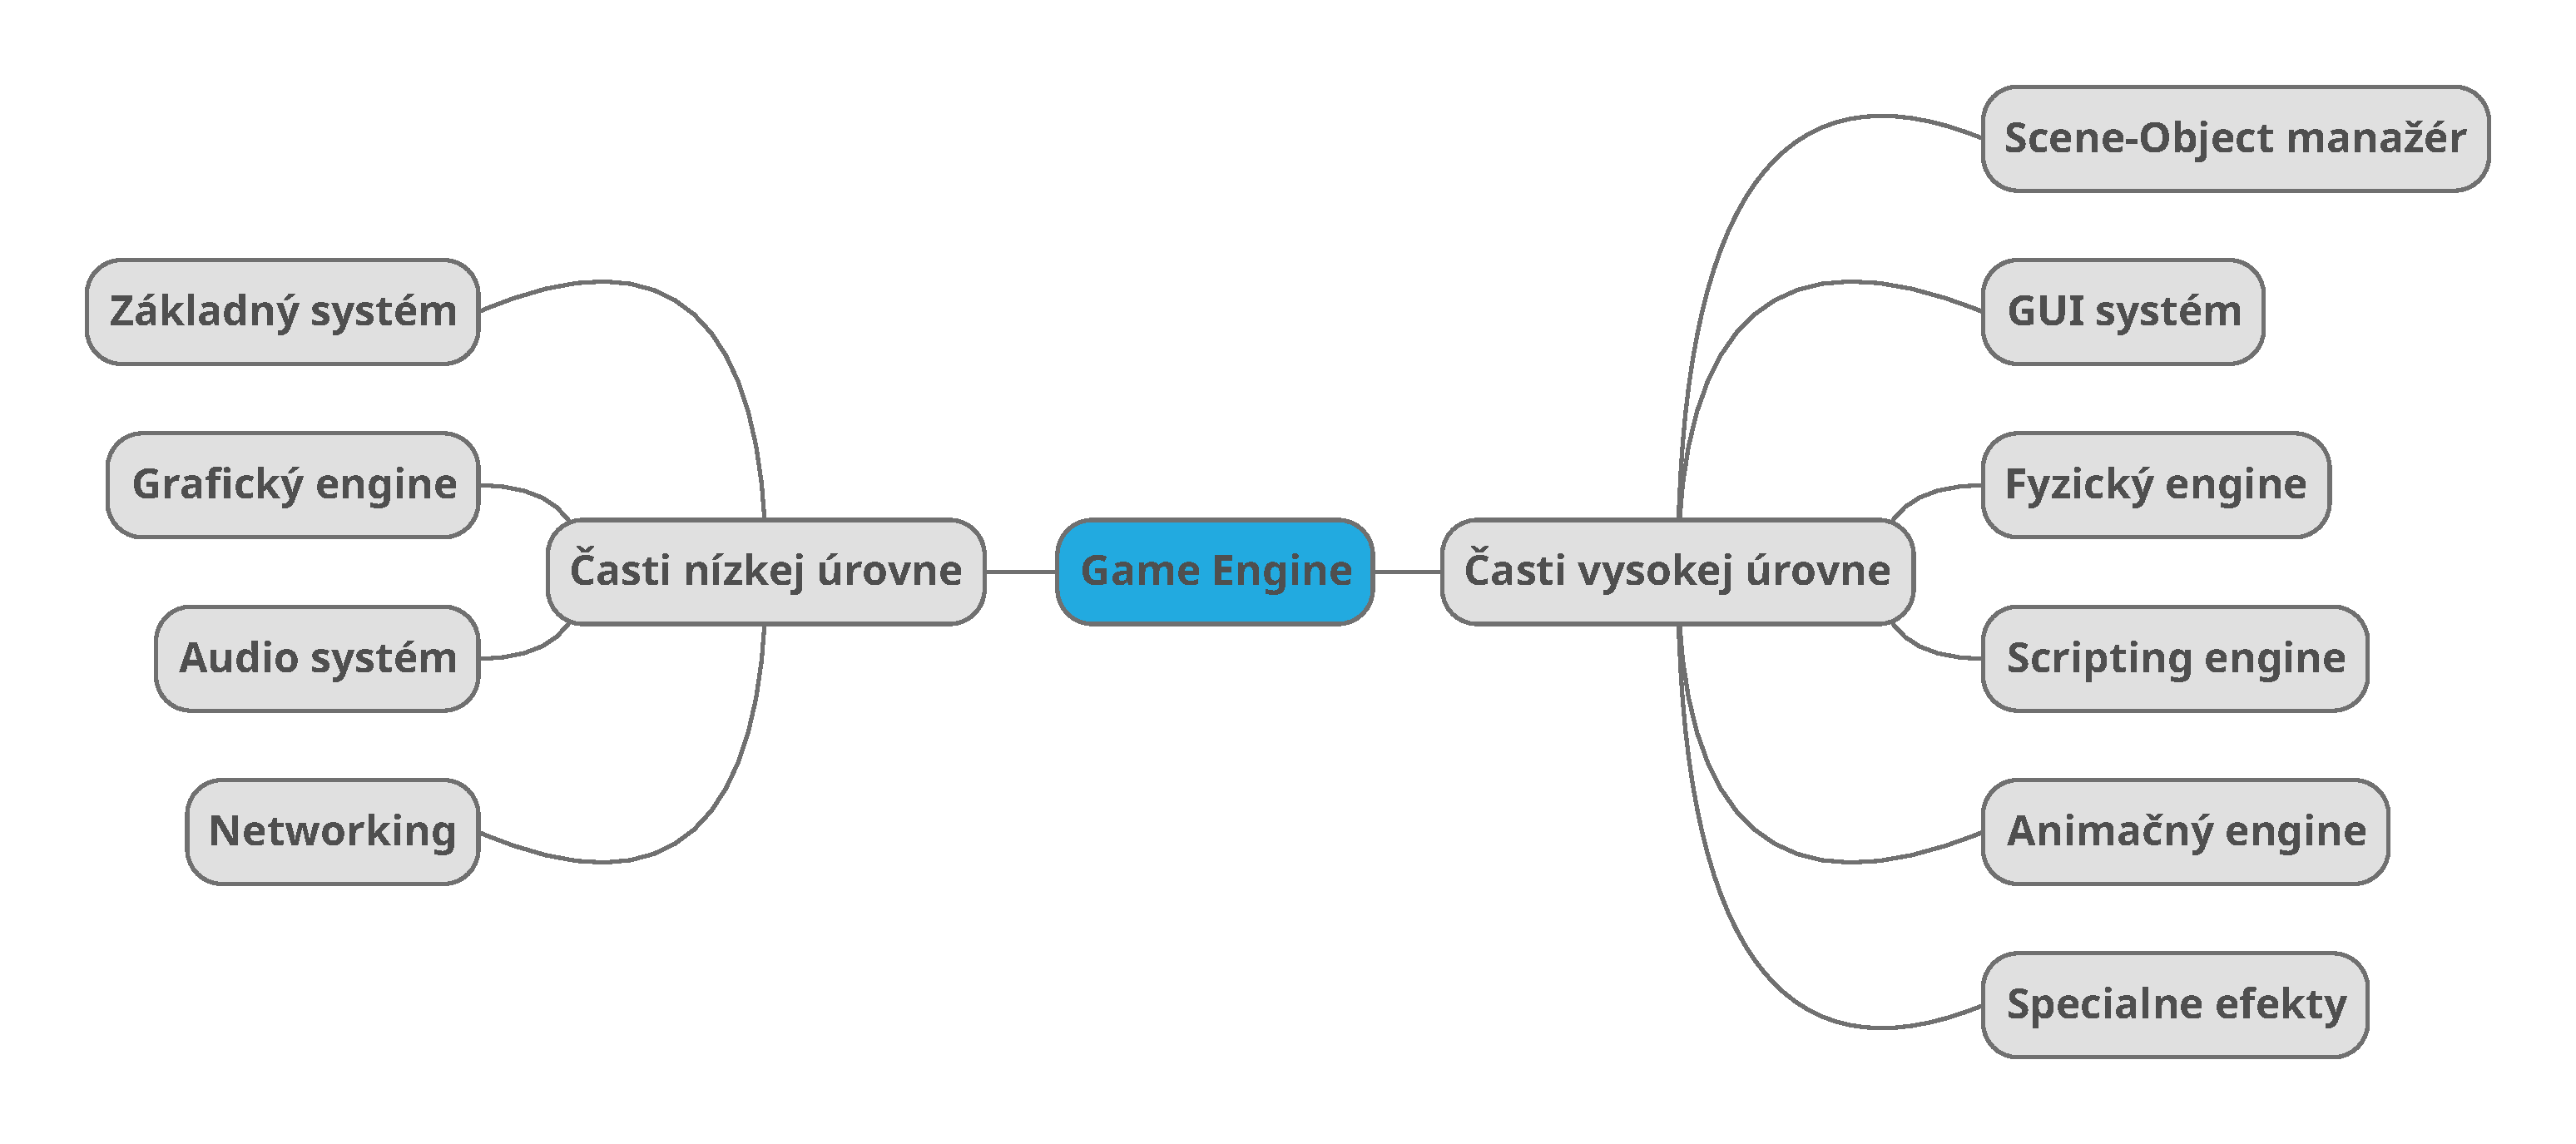
\includegraphics[width=12cm]{sys_arch}
	\subsection{Časti nízkej úrovne}
		\subsubsection{Základný systém}
			Základný systém je vlastne skupina nástrojov game engina. Sú to rôzne nástroje a softvér ako sú napríklad matematická knižnica, knižnica na operáciu s reťazcami, správa asynchrónneho čítania a zápisu súborov, dátové štruktúry, systém na správu vstupov, a mnohé iné. Z uvedených príkladov vieme povedať, že najvýznamnejšia je matematická knižnica, ktorá nám okrem základných a zložitých matematických operácií a trigonometrických funkcií poskytuje aj funkcie na operácie s vektormi a maticami. Tie sú významné hlavne v grafickom a fyzickom engine. Taktiež významné sú aj dátové štruktúry a systém na správu vstupov. Často používané dátové štruktúry sú stack, queue a Binary Search Tree(BST). Stack pracuje na princípe FILO(First In, Last Out) a queue na princípe FIFO(First In, First Out). Binary Search Tree(BST) je vlastne binary tree, kde do každého uzla s hodnotou x je z ľavej strany pripojený iba uzol s menšou hodnotou ako x a s pravej strany iba uzol s väčšou alebo rovnakou hodnotou ako x. To nám umožňuje veľmi rýchle prehľadávanie. Časová zložitosť prehľadávania v BST je O($log_2n$) a v najhoršom prípade O($n$).
		\subsubsection{Grafický engine}
			Grafický systém(Renderer) sa považuje za najzložitejší modul game enginov. Problematika v tejto oblasti spočívala v rýchlosti priestorového kreslenia obrázkov v čo najväčšom počte a za čo najmenší čas. To bolo dlhú dobu obmedzené technológiu hardvéru. V dnešnej dobe je to už menším problémom. Technológie priestorového kreslenia sú veľmi vyspelé v rýchlosti, ale sú aj oveľa realistickejšie. Veľmi známe spôsoby priestorového kreslenia sú Ray Casting a Raz Tracing. Ray Casting je menej náročná metóda a preto sa bežne používa vo video hrách. Ray Tracing je metóda, pomocou ktorej vieme nakresliť foto-realistické obrázky. Pri kreslení berie do úvahy reflekciu a refrakciu lúčov čo znamená, že priesvitné materiáli ako je sklo, budú potrebovať omnoho viac výpočtov, ale bez toho by sme foto-realizmu nevedeli replikovať. Jednou s výhod v grafickom programovaní je, že vieme písať programy ktoré sa vykonávajú na grafickej karte. Taktiež vieme preposlať dáta týkajúce sa našej scény na operačnú pamäť grafickej karty, tým zmenšujeme množstvo dát, ktoré posielame grafickej karte za jeden cyklus. To znamená že môžeme grafickej karte posielať aj matice lineárnych a nelineárnych transformácií. Potom sa výpočty robia na grafickej karte paralelne pre každý bod v našom virtuálnom priestore.
		\subsubsection{Audio systém}
			Zvuk v game enginoch je rovnako dôležitý ako grafika. Hudba a iné zvukové efekty ako sú ambientné zvuky ovplyvňujú emócie hráča a tým zlepšujú jeho zažitie hry.
		\subsubsection{Networking}
			Sieťovanie je kritickou časťou na implementáciu multiplayer možnosti. Väčšina úspešných hier sú spoločenské hry, tímové hry alebo individuálne hry pre viacero hráčov(FFA - Free For All). Známe sú aj hry MMOG(Massively Multiplayer Online Games), ktoré umožňujú veľkému množstvu hráčov, hrať súčasne. Sieťovanie nám umožňuje tvorbu serverových programov pre herné serveri a klientových programov pre hráčov.
	\subsection{Časti vysokej úrovne}
		\subsubsection{Scene-Object manažér}
			V game enginoch potrebujeme ukladať a spravovať objekty našej hre niekde v pamäti. Jednou s organizačnou metódou je Entity-Component System(ECS) \cite{ECS}. Tento systém funguje tak, že všetko v našom virtuálnom priestore sa dá reprezentovať nejakým objektom(Entity) a na základe toho aké vlastnosti chceme, aby náš objekt obsahoval prideľujeme mu jeho komponenty (Component). Môže to byť kamera, zvukový zdroj, svetlo, skriptá ktoré definuje jeho správanie a iné.
		\subsubsection{GUI systém}
			Poskytuje možnosti tvorby grafických rozhraní, rôzne menu, nastavenia a HUDs(Heads-Up Displays). Využíva modul nízkej úrovne, grafický engine na zobrazenie grafických rozhraní na obrazovku. Využíva dátovú štruktúru stack, poskytnutú od základného systému na uchovávanie stavov menu grafických rozhraní.
		\subsubsection{Fyzický engine}
			Fyzický engine je softvérový nástroj, ktorý využíva matematické a fyzické princípy na simuláciu pohybu a správania sa objektov vo virtuálnom prostredí. Simulujú realistické a zložité interakcie medzi predmetmi, ako sú kolízie, gravitácia, rôzne typy síl a iné fyzické fenomény.
			\paragraph{Kolízia} je hlavnou časťou fyzického enginu. Je to proces určovania kedy dva alebo viac predmetov vo virtuálnom priestore prišli do vztyku. Je to veľmi dôležité, lebo fyzickému enginu umožňuje presne simulovať dotyk/zrážky, ako je vzájomný odraz alebo prenos kinetickej energie. Algoritmy na zisťovanie kolízií sú veľmi zložité a náročné pre procesor. Preto je zvyčajne obmedzený počet výpočtov za sekundu.
		\subsubsection{Scripting engine}
			Scripting engine je softvér, ktorý nám umožňuje vyvíjať herné mechaniky, postavy a iné herné elementy pomocou skriptovacích jazykov. Najznámejšie skriptovacie jazyky sú C\#, Lua, Python, C++... Hlavne sa používajú na vývoj logiky a správania herných elementov, ako sú postavy, predmety a prostredia. Umožňuje tvorbu zložitých a dynamických mechaník, bez toho, aby vývojári museli písať kód nízkej úrovne. Z toho dôvodu je aj veľmi výhodný pre menej skúsených vývojárov, ktorý chcú tvoriť hry.
		\subsubsection{Animačný engine}
			V každej hre, či už 2D alebo 3D, je potrebne používať animáciu. Animation engine nám poskytuje všetky potrebné pomôcky na tvorbu animácií. V 2D hrách animácia je realizovaná pomocou obrázkov, ktoré sa po sebe striedajú. V 3D hrách sa používajú kostrové animácie, ktoré umožňujú animátorovi hýbať 3D charaktera pomocou kostí a kĺbov. 3D body toho modelu sa hýbu súčasne a relatívne na kosti toho modelu \cite{Secondary}.
		\subsubsection{Specialne efekty}
			Vizuálne efekty vylepšujú kvalitu video hier. Privádzajú ich k životu, často pomocou pohyblivých častíc, dynamických tieňov, hmle, rôznych svetelných efektov... Tento systém nie je pod-časťou grafického enginu, ale používa ho na kreslenie textúry, ktorú potom prekreslí cez obrázok zobrazený na obrazovke.
	\section{Aplikácia v gemifikačnej sfére}
		Herné enginy sa bežne využívajú na tvorbu video hier, ale dajú sa využívať aj pre iné účely. Napríklad, niektorú herné enginy sa využívajú pre simulácie a trénovanie programov pre stavbu, letiská a zdravotníctvo. Iné herné enginy sa používajú na tvorbu interaktívnych aplikácii pre virtuálnu realitu, napríklad pre múzea. Ďalšie herné enginy sa používajú v výskumoch a edukácii. Taktiež sú aj umelci, ktorý využívajú herné enginy na tvorbu umeleckých aplikácii, či už interaktívnych alebo nie. Skratka herné enginy sa dajú využívať v rôznych sférach nie len pre tvorbu video hier.
	\section{Záver}
		Tak povedali sme si čo sú game enginy, o moderných game enginoch, základných častiach game enginov nevyhnutných na tvorbu úspešných hier a o využití game enginov v gemifikačnej sfére. Pre zhrnutie, game enginy sú nástroje určené na tvorbu video hier, či už 2D alebo 3D. Poskytujú veľa rôznych pod nástrojov, potrebných na tvorbu grafických rozhraní, animácií, samotnej grafiky, zvuku... Čo sa týka využitia herných enginov, vieme že okrem tvorbe video hier, používajú sa aj pre iné účely, ako sú napríklad: interaktívne aplikácie, simulácie, trénovanie, rôzne výskumy...
		\paragraph{}Tak, ako bolo spomenuté v abstrakte tohoto článku, dostali sme sa od vzniku prvej hry\cite{FirstGame}, prvej 3D hry\cite{First3DGame} ku vzniku herných enginov a postupne k súčasným moderným hrám, ktoré by bez existencie herných enginov nenapĺňali náš každodenný život zábavou a vedomosťami.
	\section{Reakcia na témy z prednášok}
		\paragraph{Prednaška o Git-e}
			O gite som sa dozvedel ešte dávno, vtedy sa mi to zdalo dosť zložité a nerozumel som tomu. Z toho dôvodu som nemal rád git a povedal som si že sa ho nebudem učiť až kým to nebudem musieť. Na prednáške sme sa dozvedeli čo git je a ako ho používať. Kvôli jednoduchému vysvetleniu na prednáške ale aj na cvičení, bez problémov som pochopil a naučil sa používať git. Nezmenilo to môj názor, že je zbytočné používať git pre samostatné práce, ale pre tímové práce a projekty git určite používať budem.
		\paragraph{Načo budem inžinierom?}
			Táto prednáška mala na mňa najväčší vplyv, lebo ma donútila zamyslieť sa nad budúcnosťou a rozšírila mi pohľad nad možnosťou zamestnania sa. Dostali sme jednoduchú otázku, že čím chceme byť po ukončení inžinierskeho štúdia. Boli sme ticho, tak pán Kotuliak ponúkol zopár odpovedí: programátori, návrhári... Mojou pôvodnou odpoveďou bolo, že chcem byť programátorom, ale neskôr nám bolo vysvetlené, že aby sme boli programátori nepotrebujeme inžinierske štúdium a že by bola škoda nezaujímať sa nad inými možnosťami zamestnania sa s inžinierskym titulom. Ešte sme sa dozvedeli, informácie a rozdiely medzi bakalárom a inžinierom.
		\paragraph{Kreatívne písanie}
			Ja seba považujem ako menej kreatívnu osobu a kreatívne písanie mi nikdy moc nešlo. Na tejto prednáške sme sa dozvedeli o základných metódach na zlepšenie kreatívneho písania. Bohužiaľ som nemohol byť prítomný do konca prednášky, ale spomenuté metódy sme si vyskúšali na nasledujúcom cvičení. Hlavne sa mi páčilo, že sme neboli odsudzovaný podľa toho čo sme napísali, čo mi dalo vôľu písať viacej.	
	
	
	%\acknowledgement{Ak niekomu chcete poďakovať\ldots}
	
	
	% týmto sa generuje zoznam literatúry z obsahu súboru literatura.bib podľa toho, na čo sa v článku odkazujete
	\pagebreak
	\bibliography{literatura}
	\bibliographystyle{plain} % prípadne alpha, abbrv alebo hociktorý iný
\end{document}
